\documentclass[tikz,border=10pt]{standalone}
\usepackage{tikz}
\usepackage{amsmath}
\usepackage{amssymb}

% TikZ libraries
\usetikzlibrary{calc}
\usetikzlibrary{positioning}

% Custom commands for mathematical notation
\newcommand{\cS}{\mathcal{S}}
\newcommand{\R}{\mathbb{R}}
\newcommand{\vx}{\boldsymbol{x}}
\newcommand{\norm}[1]{\left\|#1\right\|}
\newcommand{\dist}{\mathrm{dist}}
\newcommand{\set}[1]{\left\{#1\right\}}

\begin{document}
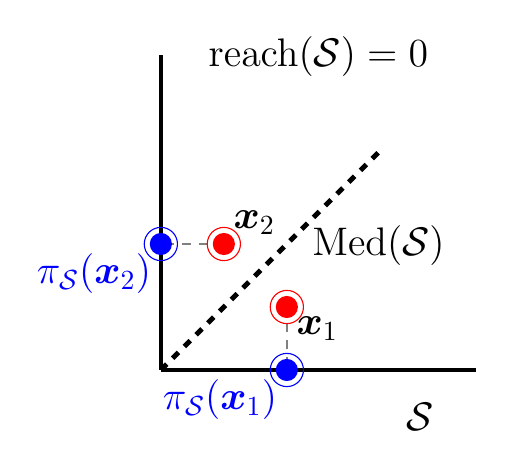
\begin{tikzpicture}[scale=2, font=\Large]
  % Define the square corner coordinates
  \coordinate (corner) at (0,0);
  \coordinate (right) at (2,0);
  \coordinate (up) at (0,2);

  % Draw the square corner (L-shape)
  \draw[black, line width=1.2pt] (corner) -- (right);
  \draw[black, line width=1.2pt] (corner) -- (up);

  % Draw the medial axis (diagonal from corner)
  \draw[black, dashed, line width=1.8pt] (corner) -- (1.4, 1.4);

  % Define two points symmetrically placed around the diagonal
  \coordinate (p1) at (0.8, 0.4);  % Below diagonal
  \coordinate (p2) at (0.4, 0.8);  % Above diagonal

  % Calculate projections
  % For p1: closer to horizontal line
  \coordinate (proj1) at (0.8, 0);
  % For p2: closer to vertical line
  \coordinate (proj2) at (0, 0.8);

  % Draw projection lines (dashed)
  \draw[dashed, gray, line width=0.8pt] (p1) -- (proj1);
  \draw[dashed, gray, line width=0.8pt] (p2) -- (proj2);

  % Draw points
  \fill[red] (p1) circle (2pt);
  \fill[red] (p2) circle (2pt);

  % Draw projected points
  \fill[blue] (proj1) circle (2pt);
  \fill[blue] (proj2) circle (2pt);

  % Labels for points
  \node[below right] at (p1) {$\boldsymbol{x}_1$};
  \node[above right] at (p2) {$\boldsymbol{x}_2$};

  % Labels for projected points
  \node[below left, blue] at (proj1) {$\pi_{\mathcal{S}}(\boldsymbol{x}_1)$};
  \node[below left, blue] at (proj2) {$\pi_{\mathcal{S}}(\boldsymbol{x}_2)$};

  % Label the medial axis
  \node[above right] at (0.9, 0.6) {$\mathrm{Med}(\mathcal{S})$};

  % Label the set
  \node[right] at (1.5, -0.3) {$\mathcal{S}$};

  % Add note about zero reach
  \node[above] at (1, 1.8) {$\mathrm{reach}(\mathcal{S}) = 0$};

  % Add small circles around points for emphasis
  \draw[red, thin] (p1) circle (3pt);
  \draw[red, thin] (p2) circle (3pt);

  \draw[blue, thin] (proj1) circle (3pt);
  \draw[blue, thin] (proj2) circle (3pt);

\end{tikzpicture}
\end{document}
